\documentclass[a4paper]{article}
\usepackage{amsfonts}
\usepackage{amsmath}
\usepackage{amssymb}
\usepackage{graphicx}     

\begin{document}
  
\noindent \large Auteur: Jeremi Lorek\\
\noindent \large Studierichting: Informatica\\
\noindent \large Oefeningenreeks 3H nr. 12.6\\

\medskip
\normalsize

$r = 2 + \cos 2\theta$ \\

beperkt domein: $[0,2\pi]$ \\

$r = 0 \Leftrightarrow \cos 2\theta = -2 \Rightarrow$ geen nulpunten. \\

$r' = 0 \Leftrightarrow -2\sin 2\theta = 0 \Leftrightarrow \sin 2\theta = 0$ \\

$\Leftrightarrow 2\theta = k\pi \Rightarrow \theta = \frac{k\pi}{2}, k \in \mathbb{Z}$ \\

\begin{tabular}{c|ccccccccc} 

	$\theta$   & $0$  &  & $\dfrac{\pi}{2}$ &  & $\pi$  &  & $\dfrac{3\pi}{2}$ &  & $2\pi$ \\ \hline
        
	$r$        & $+$  & $+$  & $+$  & $+$  & $+$  & $+$  & $+$  & $+$  & $+$ \\

	$r'$       & $0$  & $-$  & $0$  & $+$  & $0$  & $-$  & $0$  & $+$  & $0$ \\ \hline

	$r$        & $M(3)$  & $\searrow$  & $m(1)$  & $\nearrow$  & $M(3)$  & $\searrow$  & $m(1)$  & $\nearrow$  &$M(3)$  \\

\end{tabular} \\


\begin{figure}[h]
\centering
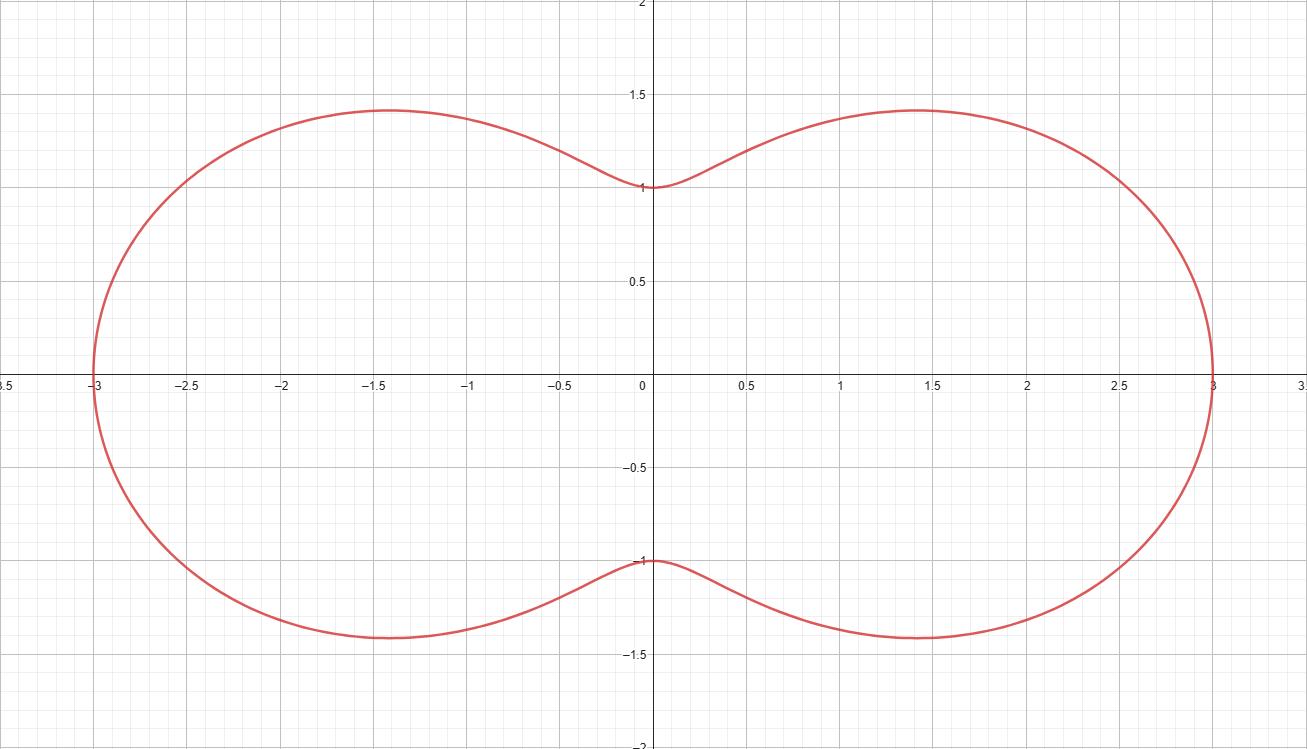
\includegraphics[width=10cm]{3H-12.6-jeremi.lorek.INF.png} \\
\end{figure}

\begin{thebibliography}{999}
%\bibitem{a} Referentie
\end{thebibliography}

\end{document}
